Энэ бүлэгт судалгааны ажлын үндэслэл, хүрэх зорилго болон зорилтуудыг танилцуулна.
\section{Сэдэв сонгосон үндэслэл}
Вэб аппликейшн хөгжүүлэлтэд орчин үеийн JavaScript фреймворкууд өргөн ашиглагдаж байгаа хэдий ч, зарим тохиолдолд серверийн талд рендер хийгддэг уламжлалт технологитой хослуулан ашиглах шаардлага гардаг. Ийм ялгаатай технологийн парадигмуудыг нэгтгэж нэгдсэн хэрэглэгчийн интерфейс үүсгэх нь архитектурын хувьд хүндрэлтэй байдаг. Иймд шинээр хөгжүүлэгдэж буй МУИС-ийн Дипломын ажлын удирдлагын системийн хөгжүүлэлтийн нэгэн хувилбар болгон холимог микрофронтенд архитектурыг сонгон авч, React, JSF фреймворкуудыг хэрхэн уялдуулан ажиллуулж болохыг бодитоор хэрэгжүүлэн, туршилт хийж судлах нь энэхүү сэдвийг сонгох үндэслэл болсон болно.
\section{Зорилго}
	\quad \quad	МУИС-ийн Дипломын ажлын удирдлагын системийн хэрэглэгчийн интерфейс дээр React болон JSF технологийг хослуулсан микрофронтенд архитектурыг туршина.
\section{Зорилт}
	Дээрх зорилгод хүрэхийн тулд дараах зорилтуудыг дэвшүүлэн ажиллана. Үүнд:
\begin{enumerate}
	\item Судалгаа хийх зорилтоор микрофронтенд архитектурын онол, арга зүйг судлах;
	\item Туршилтын загвар боловсруулах зорилтоор React, JSF ашиглан холимог архитектур бүхий системийн туршилтын загварыг хөгжүүлэх;
	\item Туршилт ба үнэлгээ хийх зорилтоор боловсруулсан загвар дээрээ туршилт хийж, ISO/IEC 25010 стандарт болон DORA, ATAM аргачлалаар үнэлж, дүгнэнэ.
\end{enumerate}

\section{Сэдвийн судлагдсан байдал}
Энэхүү судалгаанд Scopus болон DiVA сангаас микрофронтенд архитектурын чиглэлээрх 10 гол бүтээлийг сонгон авч шинжиллээ. Үр дүнг хүснэгт \ref{tab:related_work_summary}-д нэгтгэв.

\begin{itemize}
\item Интеграцийн шийдэл: \cite{mannisto2023, pavlenko2020} нар систем задлах онолыг судалсан ч Strangler Fig үлгэр загварын шилжилтийн үе болох төлөв хадгалдаг болон төлөвгүй  архитектурыг зэрэгцүүлэн ажиллуулах техникийн зааварчилгааг орхигдуулсан байна.
\item Нөөцийн давхардал: \cite{ameer2024, taibi2022} зэрэг судалгаанууд сүлжээний ачааллыг хэмжсэн боловч холимог орчин дахь серверийн нөөцийн давхардал, түүний нөлөөллийг тооцоолоогүй байна.
\item Парадигм хоорондын төлөв: \cite{silva2024, mohammed2022} нар төлөв хуваалцахыг гол сорилт гэж онцолсон ч ялгаатай парадигм бүхий системүүдийг уялдуулах бодит техникийн шийдлийг санал болгоогүй.
\item Танин мэдэхүйн ачаалал: \cite{bjelotomic2024, tilak2020} зэрэг бүтээлүүд хөгжүүлэлтийн хурдыг хэмжсэн ч хоёр өөр технологийг нэгэн зэрэг удирдах үед хөгжүүлэгчид үүсэх танин мэдэхүйн ачааллыг үнэлээгүй орхисон байна.
\end{itemize}

\section{Судалгааны шинэлэг тал}
Энэ бакалаврын судалгааны ажлын шинэлэг тал нь дараах хоёр хэсгээс бүрдэнэ. Үүнд:
\begin{enumerate}
    \item Серверийн талын JSF болон клиент талын React фреймворкийг \texttt{<script>} интеграци ашиглан DOM түвшинд нэгтгэсэн туршилтын загвар хөгжүүлсэн.
    \item Хэрэгжүүлсэн холимог микрофронтенд архитектурыг ISO/IEC 25010 чанарын стандартын дагуу үнэлж дүгнэсэн.
\end{enumerate}
\section{Судалгааны ажлын үр дүн}
\subsubsection{Үр дүн}
\hspace*{0.6cm}Энэ судалгааны хүрээнд JSF, React фреймворкуудыг хослуулсан микрофронтенд архитектурын туршилтын загварыг хэрэгжүүлж, модулиудыг бие даан ажиллуулж, интеграци хийх боломжтойг харуулна. Мөн , үнэлгээний үр дүнг гаргана.
\subsubsection{Ач холбогдол}
\hspace*{0.6cm}Энэ судалгаа нь өөр өөр технологийн стэк бүхий хэрэглээний программуудыг микрофронтенд архитектураар хэрхэн нэгтгэх техникийн шийдлийг бодитоор харуулсан кейс судалгаа болно. Цаашид ижил төстэй технологийн хоршил ашиглах хэрэгцээ гарсан оюутнуудад техникийн лавлагаа, харьцуулалт хийх суурь мэдээлэл болох ач холбогдолтой юм.

\section{Судалгааны ажлын арга зүй}
Судалгааны үйл явцыг илүү сайн ойлгохын тулд 5 үе шатанд хуваасан. Үе шат бүрд дараагийн шатанд бэлтгэх, хэрэгжүүлэлтийн талаар туршлага хуримтлуулах, үүссэн өгөгдлийг хэмжиж, цуглуулах тодорхой үйлдлүүдийг гүйцэтгэнэ. Зураг \ref{fig:phases}-д судалгааны үйл явцын үе шатууд болон тэдгээрийг хэрэгжүүлэх дарааллыг харуулав.
\subsubsection{Сэдвийн судлагдсан байдал, хүрээг тодорхойлох}
\hspace*{0.6cm}Энэ үе шатны зорилго нь сэдвийн ойлголттой танилцахад оршино. Шаардлагатай мэдлэгийн түвшинд хүрэхийн тулд Scopus, DiVA (Дэд бүлэг \ref{sec:literature-review}-ыг үзнэ үү) өгөгдлийн сангаас гадна төрөл бүрийн блог, форум, фреймворкүүдийн техникийн баримт бичгүүдийг ашигласан. Энд ISO/IEC 25010 стандартыг судалж, МУИС-ийн Дипломын ажлын удирдлагын системд шаардлагатай байж болох программ хангамжийн чанарын үзүүлэлтүүдийн тодорхойлолтыг гаргасан.
\subsubsection{Туршилтын загвар}
\hspace*{0.6cm}Фронтенд хөгжүүлэлтэд микрофронтенд архитектурыг хэрэгжүүлэх техникийн мэдлэг, туршлага хуримтлуулах зорилгоор туршилтын загварыг (Дэд бүлэг \ref{sec:prototype}-ыг үзнэ үү) хөгжүүлсэн. Туршлага хуримтлуулахаас гадна, хэрэгжүүлэлтийн явцад төрөл бүрийн сорилт, бэрхшээлүүд гарч ирсэн болно. Туршилтын загвар нь React,JSF гэсэн хоёр өөр фреймворкоор хөгжүүлэгдсэн, микрофронтенд хэрэглээний программуудыг ачаалдаг жижиг хэмжээний хэрэглээний программ юм.

\subsubsection{Туршилт}
\hspace*{0.6cm}Туршилтын үе шат нь МУИС-ийн Дипломын ажлын удирдлагын системийн хэрэглэгчийн интерфейсийг цэвэр микрофронтенд болон холимог микрофронтенд архитектураар хөгжүүлэх үйл явцаас бүрдэнэ. Хөгжүүлэлтийн давтамж бүрийн дараа санал болгож буй шийдлийг сонгогдсон ISO/IEC 25010 чанарын үзүүлэлтүүд болон микрофронтенд архитектурын үндсэн зарчмуудтай уялдуулан үнэлэв.

\subsubsection{Кэйс судалгаа}
\hspace*{0.6cm}Кэйс судалгааны объект нь МУИС-ийн Дипломын ажлын удирдлагын систем бөгөөд харьцуулах хоёр хувилбарыг тодорхойлов: нэгдүгээрт, JSF~2.2 монолит архитектур; хоёрдугаарт, Vite Module Federation ашиглан хэрэгжүүлсэн React MFE болон Spring WebFlux реактив микросервис архитектур. Судалгааны нэгж нь нэг системийн хоёр архитектурын хувилбарыг ижил функциональ шаардлага, ижил туршилтын орчинд (Apple M2 Pro, macOS~15.3, localhost) хэмжсэн нэг кэйс зохиомж юм. Хэмжигдэх үзүүлэлтүүдийг дөрвөн бүлэгт хуваав: хөгжүүлэлтийн хурд (Lead Time, HMR/reload), ажлын ачааллын гүйцэтгэл (RAM, латенц), сүлжээний зардал (payload, кэш), кодын чанар (Cyclomatic Complexity, duplication).

\subsubsection{Өгөгдлийн шинжилгээ}
\hspace*{0.6cm}Цуглуулсан өгөгдлийг хоёр аргачлалаар шинжлэв. Нэгдүгээрт, ISO/IEC~25010 стандартын 7 чанарын үзүүлэлт (Хугацааны төлөв, Харилцан ажиллах чадвар, Модульлаг байдал, Дахин ашиглах боломж, Шинжилж болохуйц байдал, Өөрчлөх боломж, Тестлэх боломж)-ийг Google Lighthouse, SonarQube, madge, Jest, Cypress хэрэгслүүдийн тоон гаралтаар хэмжиж, JSF болон React MFE архитектурыг харьцуулан оноолов. Хоёрдугаарт, ATAM (Architecture Trade-off Analysis Method) аргачлалаар архитектурын гол шийдвэрүүдийн мэдрэмтгий цэг (Sensitivity Point) болон буулт цэгүүдийг (Trade-off Point) тодорхойлж, чанарын үзүүлэлтүүдийн хоорондох өрсөлдөөнт харилцааг шинжиллэв.

\begin{figure}[h!]
	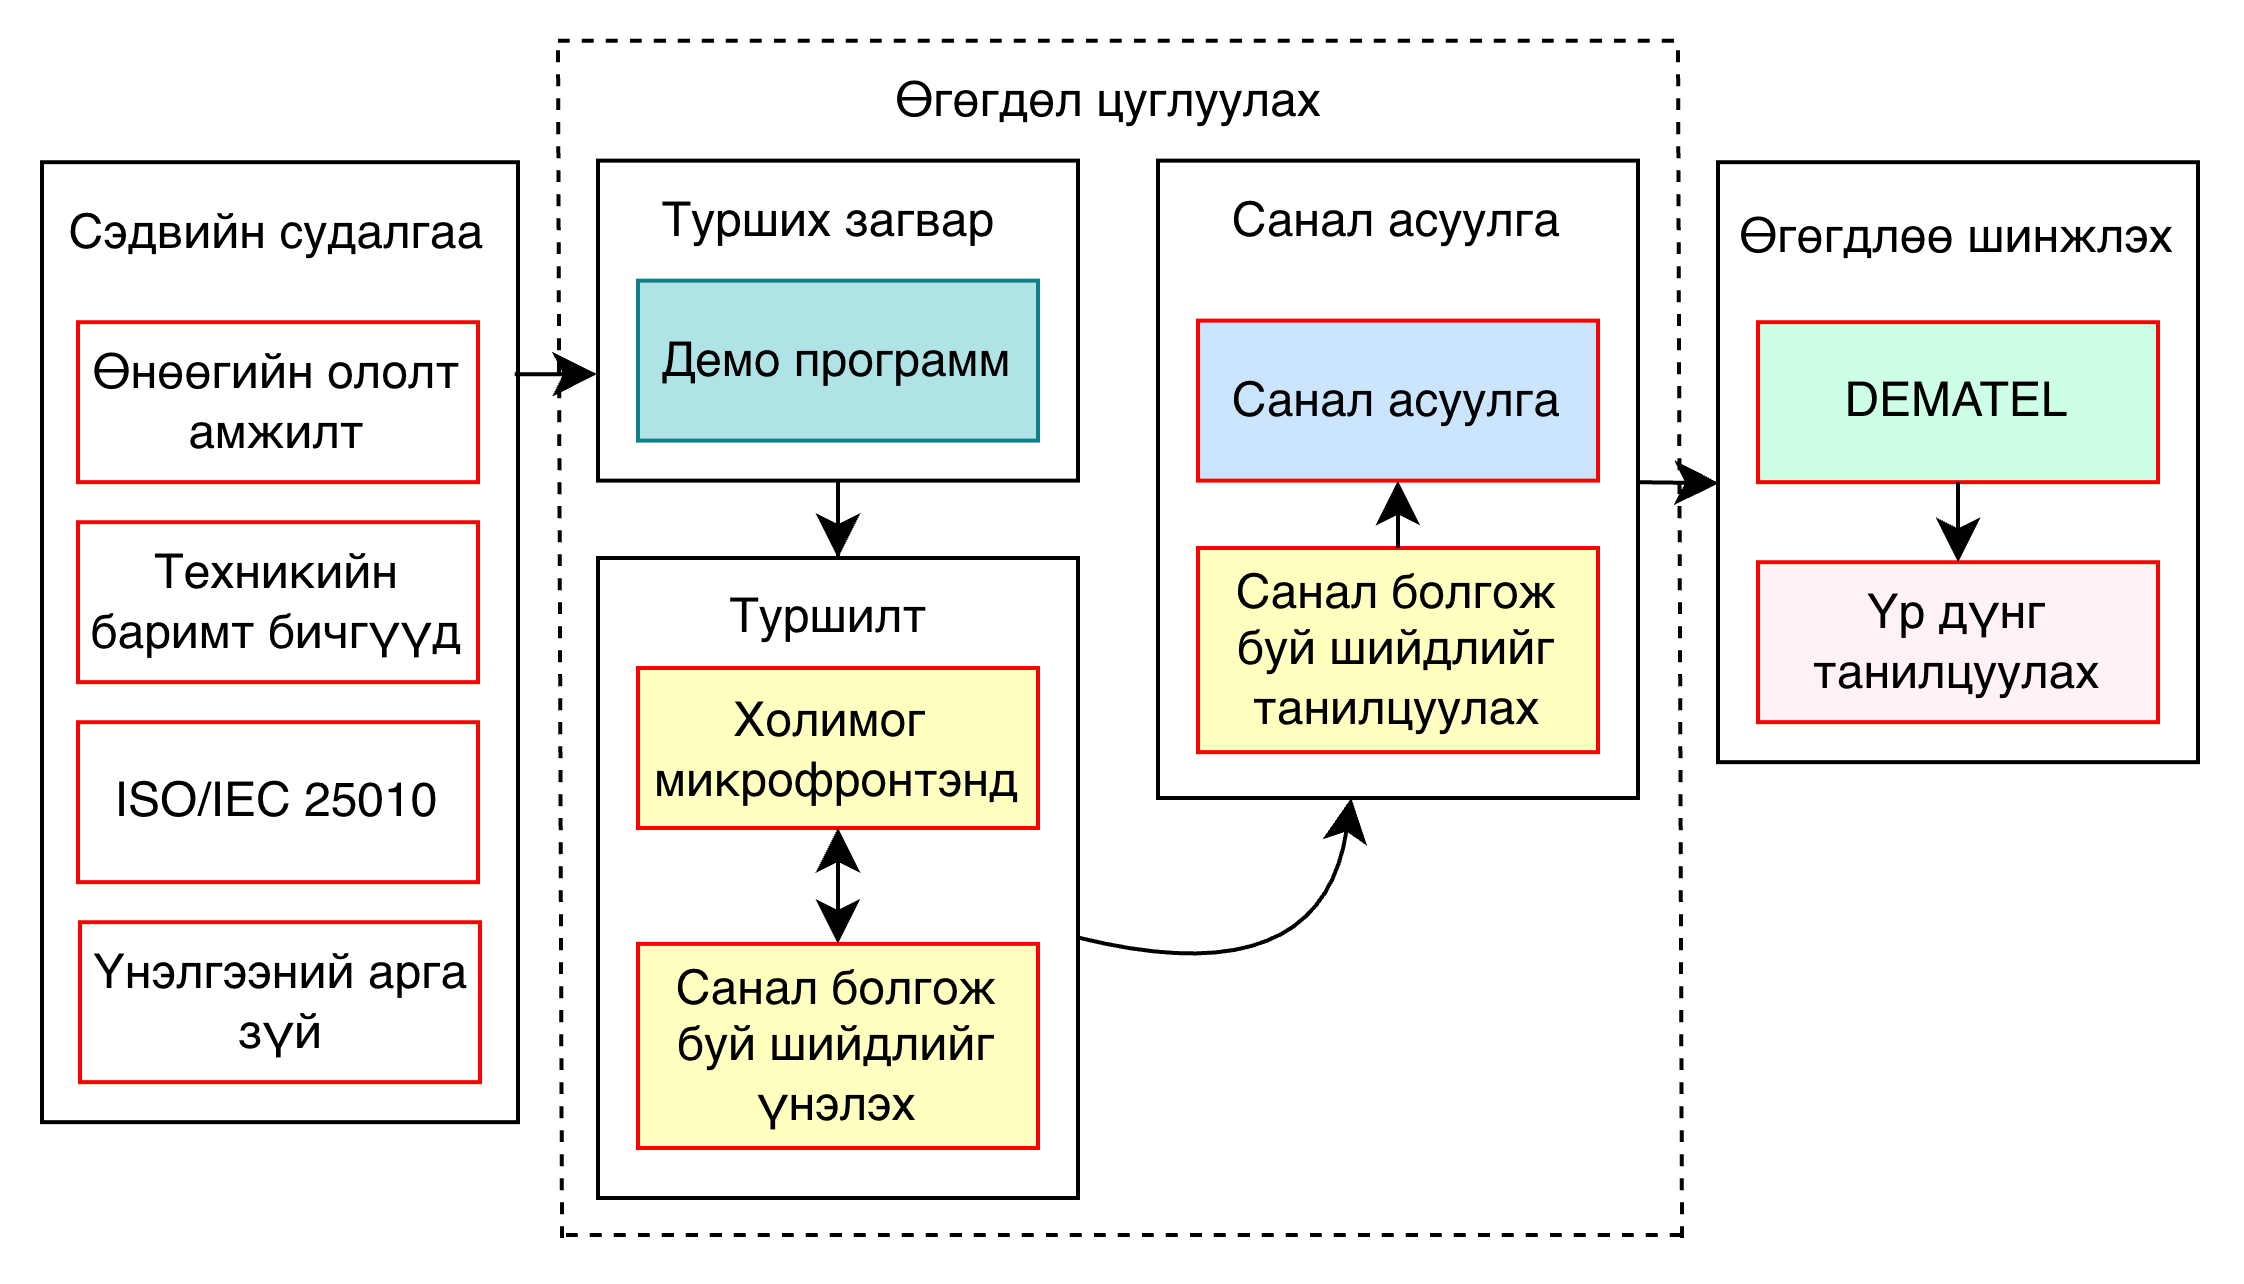
\includegraphics[width=17cm]{images/phases.png}
	\caption{Судалгааны үйл явцын үе шатууд}
	\label{fig:phases}
\end{figure}